%%%%%%%%%%%%%%%%%%%%%%%%%%%%%%%%%%%%%%%%%%%%%%%%%%%%%%%%%%%%%%%%%%%%%%%%%%%%%%%%%%
\begin{frame}[fragile]\frametitle{Abstract}

Graph query languages, while precise and powerful, can sometimes be challenging to comprehend and employ. 
However, employing natural language to construct and query graphs presents an ideal alternative. 
This approach is particularly suitable for Knowledge Graphs derived from textual data. 
This presentation explores the foundation, methodologies, and illustrative instances of utilizing LLMs to enhance KGs.


\end{frame}

%%%%%%%%%%%%%%%%%%%%%%%%%%%%%%%%%%%%%%%%%%%%%%%%%%%%%%%%%%%%%%%%%%%%%%%%%%%%%%%%%%
\begin{frame}[fragile]\frametitle{}
\begin{center}
{\Large Knowledge Graph (KG)}

\end{center}
\end{frame}

%%%%%%%%%%%%%%%%%%%%%%%%%%%%%%%%%%%%%%%%%%%%%%%%%%%%%%%%%%%%%%%%%%%%%%%%%%%%%%%%%%
%%%%%%%%%%%%%%%%%%%%%%%%%%%%%%%%%%%%%%%%%%%%%%%%%%%%%%%%%%%
\begin{frame}[fragile]\frametitle{What is KG?}

\begin{itemize}
\item A knowledge graph is a graph-based database that represents knowledge in a structured and semantically rich format. 
\item This could be generated by extracting entities and relationships from structured or unstructured data, such as text from documents. 
\item A key requirement for maintaining data quality in a knowledge graph is to base it on standard ontology. 
\item Having a standardized ontology often involves the cost of incorporating this ontology in the software development cycle.
\end{itemize}

\end{frame}

%%%%%%%%%%%%%%%%%%%%%%%%%%%%%%%%%%%%%%%%%%%%%%%%%%%%%%%%%%%
\begin{frame}[fragile]\frametitle{Populating KG}

\begin{center}
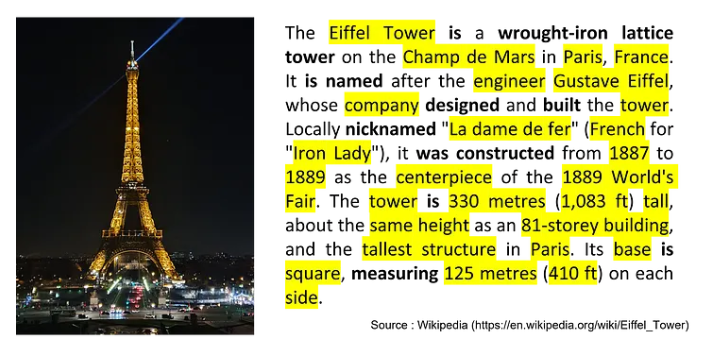
\includegraphics[width=\linewidth,keepaspectratio]{llm48}
\end{center}

{\tiny (Ref: Automatic Knowledge Graphs: The Impossible Grail - Patrick Meyer)}

\end{frame}

%%%%%%%%%%%%%%%%%%%%%%%%%%%%%%%%%%%%%%%%%%%%%%%%%%%%%%%%%%%
\begin{frame}[fragile]\frametitle{Populating KG}

\begin{itemize}
\item The Eiffel Tower is a wrought-iron lattice tower.
\item The Eiffel Tower is located on the Champ de Mars.
\item The Champ de Mars is located in Paris.
\item Paris is located in France.
\item The Eiffel Tower is named after the engineer Gustave Eiffel.
\item Gustave Eiffel’s company designed the Eiffel Tower.
\item Gustave Eiffel’s company built the Eiffel Tower.
\item The Eiffel Tower is locally nicknamed “La dame de fer”.
\item “La dame de fer” is the French for ”The Iron Lady”
\item The Eiffel Tower was constructed from 1887 to 1889.
\item The Eiffel Tower was constructed as the centerpiece of the 1889 World’s Fair.
\item The Eiffel Tower is 330 meters high.
\item The Eiffel Tower is the same height as an 81-storey building.
\item The Eiffel Tower is the tallest structure in Paris.
\item The base of the Eiffel Tower is a square.
\item The base of the Eiffel Tower measures 125 meters on each side.epresenting conceptual understanding, establishing connections between the LLM's numerical vectors and the KG's ontological classes.
\end{itemize}

{\tiny (Ref: Automatic Knowledge Graphs: The Impossible Grail - Patrick Meyer)}

\end{frame}

%%%%%%%%%%%%%%%%%%%%%%%%%%%%%%%%%%%%%%%%%%%%%%%%%%%%%%%%%%%
\begin{frame}[fragile]\frametitle{Populating KG}

\begin{center}
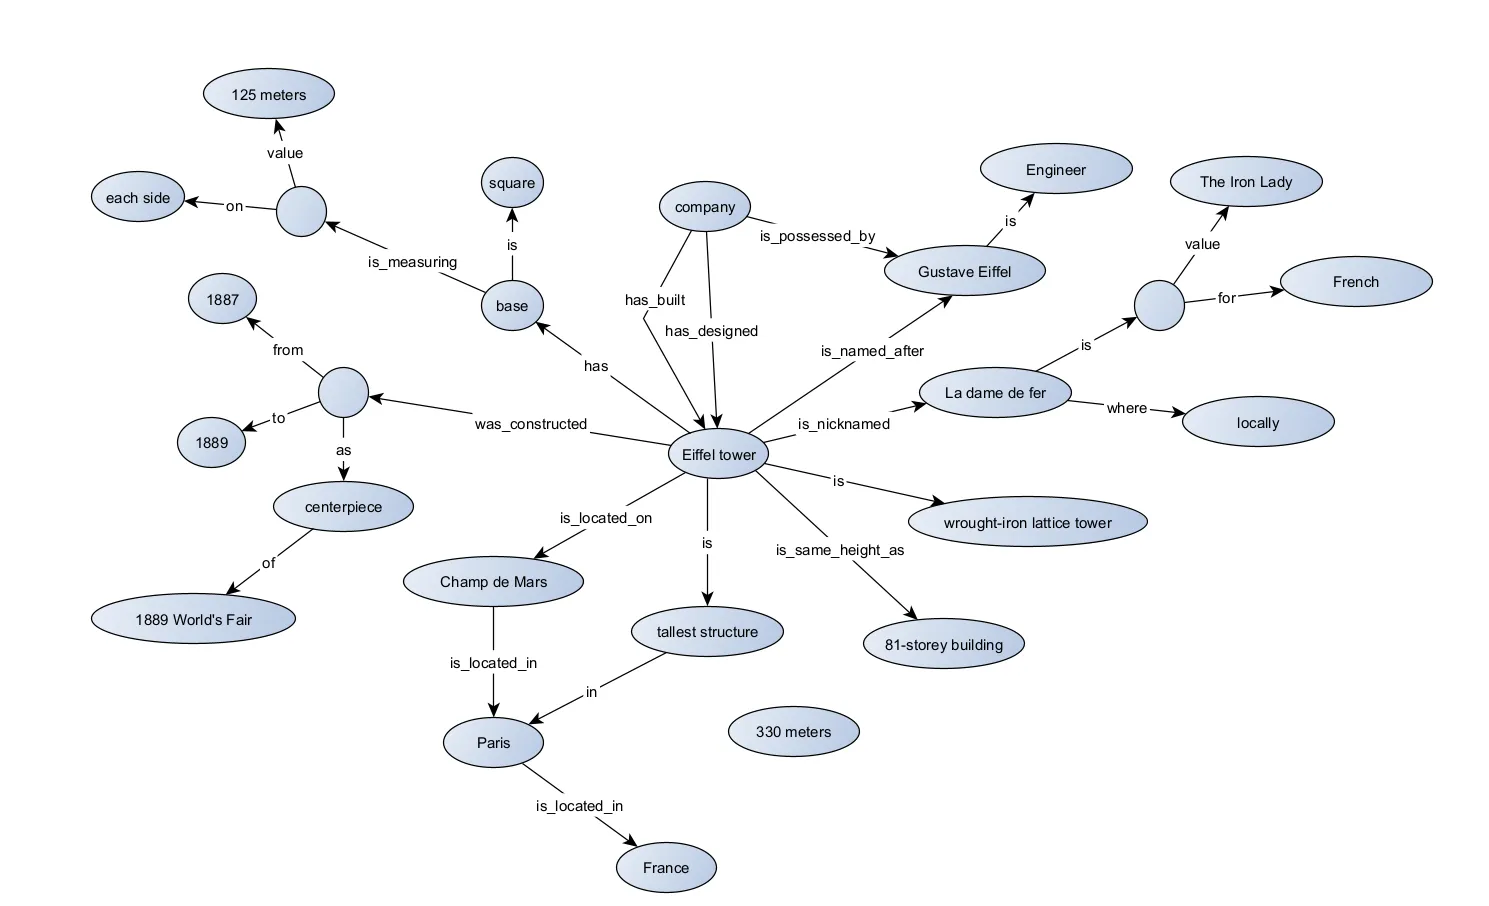
\includegraphics[width=\linewidth,keepaspectratio]{llm49}
\end{center}

{\tiny (Ref: Automatic Knowledge Graphs: The Impossible Grail - Patrick Meyer)}

\end{frame}

%%%%%%%%%%%%%%%%%%%%%%%%%%%%%%%%%%%%%%%%%%%%%%%%%%%%%%%%%%%
\begin{frame}[fragile]\frametitle{Populating KG is not easy}

\begin{center}
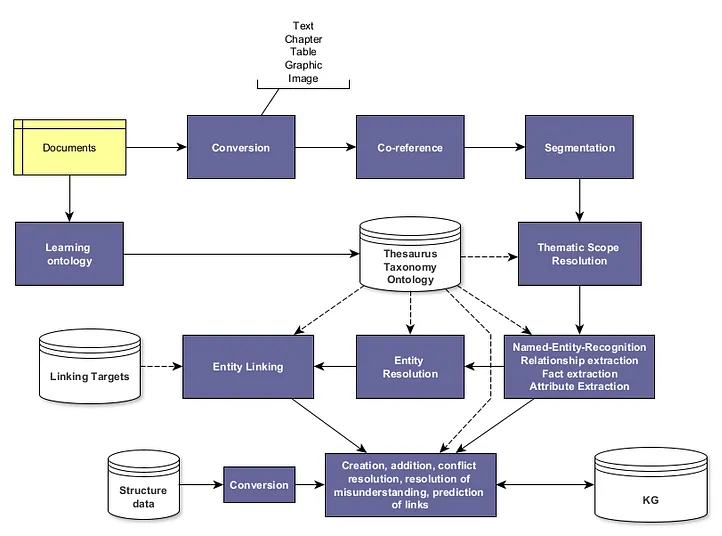
\includegraphics[width=\linewidth,keepaspectratio]{llm50}
\end{center}

{\tiny (Ref: Automatic Knowledge Graphs: The Impossible Grail - Patrick Meyer)}

\end{frame}

%%%%%%%%%%%%%%%%%%%%%%%%%%%%%%%%%%%%%%%%%%%%%%%%%%%%%%%%%%%%%%%%%%%%%%%%%%%%%%%%%%
%%%%%%%%%%%%%%%%%%%%%%%%%%%%%%%%%%%%%%%%%%%%%%%%%%%%%%%%%%%
\begin{frame}[fragile]\frametitle{What is LLM?}

\begin{itemize}
\item Large Language Models (LLMs) are machine learning algorithms to interpret, translate, and summarize natural language texts. The size of large language models generally spans hundreds of gigabytes with trillions of parameters.cle.
\item These models use deep neural networks to learn from extensive training data for generating appropriate outputs. By implementing the self-attention mechanisms of a transformer architecture, a large language model can relate words in a sentence, even if the words are positioned incorrectly. The relationships between words are captured by assessing and comparing the attention scores of every word in a text sequence. The training text data for large language models is accumulated from multiple sources - depending on the type, such as books, open internet, articles, social media, or research papers. 
\item Large language models are used in a wide range of applications as conversational AI, content creation engines, search engines, customer service agents, and more. They are a powerful innovation designed to automate and enhance natural language processing tasks.
\end{itemize}

\end{frame}


%%%%%%%%%%%%%%%%%%%%%%%%%%%%%%%%%%%%%%%%%%%%%%%%%%%%%%%%%%%%%%%%%%%%%%%%%%%%%%%%%%
\begin{frame}[fragile]\frametitle{}
\begin{center}
{\Large Knowledge Graph + Language Model}

\end{center}
\end{frame}


%%%%%%%%%%%%%%%%%%%%%%%%%%%%%%%%%%%%%%%%%%%%%%%%%%%%%%%%%%%%%%%%%%%%%%%%%%%%%%%%%%
%%%%%%%%%%%%%%%%%%%%%%%%%%%%%%%%%%%%%%%%%%%%%%%%%%%%%%%%%%%
\begin{frame}[fragile]\frametitle{How Can Knowledge Graphs and LLMs Work Together?}

\begin{itemize}
\item Combining knowledge graphs and large language models can provide a powerful solution to the limitations of an LLM's linguistic knowledge and can potentially solve the hallucination problem to improve the accuracy of query results. ural language processing tasks.
\item Integrating a knowledge graph with a large language model involves incorporating a contextual knowledge base into the model, allowing the model to make logical connections between concepts. This enables the large language model to draw on a variety of information sources, including structured and unstructured data, to generate more accurate and relevant outputs. Moreover, it allows the model to reason with greater depth of understanding and generate more meaningful text.
\end{itemize}

\end{frame}

%%%%%%%%%%%%%%%%%%%%%%%%%%%%%%%%%%%%%%%%%%%%%%%%%%%%%%%%%%%%%%%%%%%%%%%%%%%%%%%%%%
%%%%%%%%%%%%%%%%%%%%%%%%%%%%%%%%%%%%%%%%%%%%%%%%%%%%%%%%%%%
\begin{frame}[fragile]\frametitle{Why?}

\begin{itemize}
\item KnowledgeGraphs are superb at representing a domain’s data, and, together with a model, can deliver answers, though the questions need to be formulated as a query by an expert.
\item Conversely, Large Language Models (LLM) allow any user to ask a question to retrieve a comprehensive answer, but that answer will not include information drawn from the users’ domain data.
\end{itemize}
	
So, combining both will be a Win-Win situation.

{\tiny (Ref: Knowledge Graphs + Large Language Models = The ability for users to ask their own questions? - Peter Lawrence)}

\end{frame}

%%%%%%%%%%%%%%%%%%%%%%%%%%%%%%%%%%%%%%%%%%%%%%%%%%%%%%%%%%%
\begin{frame}[fragile]\frametitle{What?}

Solution: Let LLM convert verbose query to GraphQL syntax which does the information retrieval. LLM make is back into verbose answer.
	
{\tiny (Ref: Knowledge Graphs + Large Language Models = The ability for users to ask their own questions? - Peter Lawrence)}

\end{frame}

%%%%%%%%%%%%%%%%%%%%%%%%%%%%%%%%%%%%%%%%%%%%%%%%%%%%%%%%%%%
\begin{frame}[fragile]\frametitle{How?}

\begin{itemize}
\item Query : \lstinline|How is Valve-104 connected to Reflux-401?|
\item Using the OpenAI gpt-3.5-turbo LLM, provide the ontology of the RDF graph as the context prompt for the LLM.
\item Ask it to prepare some SPARQL
\end{itemize}	

\begin{lstlisting}
Sure! Here is an example of a SPARQL query that returns the sequence of nodes that connect two particular nodes, assuming that there is a unique path between them:
```
PREFIX connectivity: <http://example.org/ontology#>
SELECT ?path
WHERE {
  {
    <http://example.org/node1> (connectivity:connectedTo)+ ?path .
    ?path connectivity:connectedTo <http://example.org/node2> .
  }
}
```
\end{lstlisting}

\end{frame}

%%%%%%%%%%%%%%%%%%%%%%%%%%%%%%%%%%%%%%%%%%%%%%%%%%%%%%%%%%%
\begin{frame}[fragile]\frametitle{How?}

\begin{itemize}
\item This query uses the property path syntax to find all paths that connect the two nodes. The syntax `(connectivity:connectedTo)+` means that we are looking for one or more occurrences of the "connectedTo" property, which allows us to traverse a path of arbitrary length.
\item The query returns the variable "?path," which represents the sequence of nodes that connect the two nodes. This variable will contain a list of URIs representing the nodes in the path.
\item Note that this query assumes that there is a unique path between the two nodes. If there are multiple paths, or if there are cycles in the graph, the query may return multiple results or an incorrect result.
\end{itemize}	

\end{frame}

%%%%%%%%%%%%%%%%%%%%%%%%%%%%%%%%%%%%%%%%%%%%%%%%%%%%%%%%%%%
\begin{frame}[fragile]\frametitle{LLM + KG for Recommendations}

Augmenting company information from KG and adding it into the prompt for better results.

\begin{center}
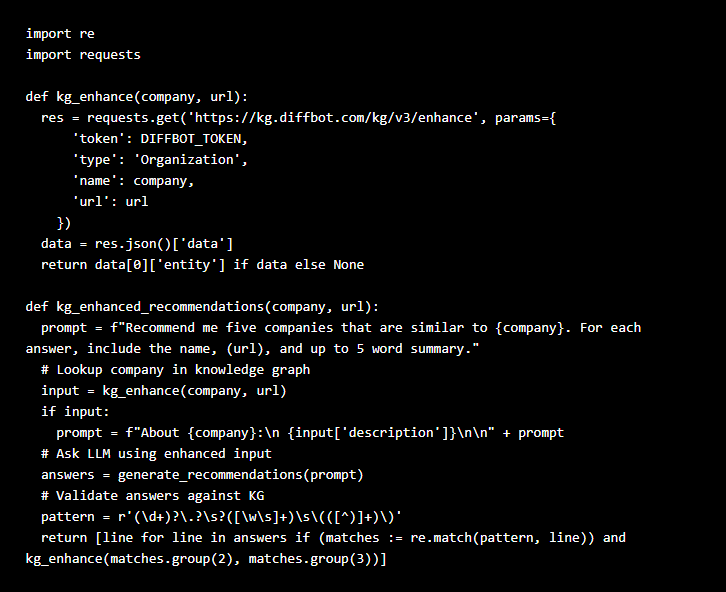
\includegraphics[width=0.5\linewidth,keepaspectratio]{llm51}
\end{center}	

{\tiny (Ref: Generating Company Recommendations using Large Language Models and Knowledge Graphs - Mike Tung)}

\end{frame}

%%%%%%%%%%%%%%%%%%%%%%%%%%%%%%%%%%%%%%%%%%%%%%%%%%%%%%%%%%%%%%%%%%%%%%%%%%%%%%%%%%
\begin{frame}[fragile]\frametitle{}
\begin{center}
{\Large Leveraging KG for Better LLM}
\end{center}
\end{frame}

%%%%%%%%%%%%%%%%%%%%%%%%%%%%%%%%%%%%%%%%%%%%%%%%%%%%%%%%%%%
\begin{frame}[fragile]\frametitle{How?}

\begin{itemize}
\item Large Language Models (LLMs), such as ChatGPT, have demonstrated immense potential in various applications but are limited by hallucinations, misinformation, and biases in enterprise contexts.
\item How integrating a graph-based Knowledge Graph as a support mechanism and interface can significantly improve the capabilities of LLMs?
\end{itemize}	

\end{frame}

%%%%%%%%%%%%%%%%%%%%%%%%%%%%%%%%%%%%%%%%%%%%%%%%%%%%%%%%%%%
\begin{frame}[fragile]\frametitle{Limitations of Large Language Models in the Enterprise Context}

\begin{itemize}
\item Hallucinations: Instances where LLMs generate plausible responses but lack factual accuracy, potentially leading to detrimental consequences in enterprise applications.
\item Misinformation: LLMs can inadvertently perpetuate false information due to their training on vast and diverse datasets containing inaccuracies.
\item Biases: LLMs may exhibit biases in their training data, resulting in prejudiced outputs that can negatively impact organizational decision-making processes.
\item Cut-off: Some LLMs are unaware of any events that happened after their training. For example, if you ask ChatGPT about an event in 2023, you will get the following response.
\item Corpus: The same problem will occur if you ask an LLM about any event not present in its training dataset ie doesn’t have any knowledge about private or confidential information that might be available even before the knowledge cutoff date.
\item At the moment, fine-tuning approaches can help mitigate hallucinations but cannot completely eliminate them. One problem is that the LLMs do not cite their sources when providing answers
\item There is no concept of access restrictions, meaning that anybody interacting with the LLM has access to all of its information.
\end{itemize}	

\end{frame}

%%%%%%%%%%%%%%%%%%%%%%%%%%%%%%%%%%%%%%%%%%%%%%%%%%%%%%%%%%%
\begin{frame}[fragile]\frametitle{Solution for Limitations}

\begin{itemize}
\item Fine-tuning an LLM, ie the supervised training phase, during which you provide additional question-answer pairs to optimize the performance of the Large Language Model (LLM).unbiased information.
\item One use case is fine-tuning a model to update and expand its internal knowledge.
\item In contrast, the other use case is focused on fine-tuning a model for a specific task like text summarization or translating natural language to database queries.
\end{itemize}	

\end{frame}


%%%%%%%%%%%%%%%%%%%%%%%%%%%%%%%%%%%%%%%%%%%%%%%%%%%%%%%%%%%
\begin{frame}[fragile]\frametitle{Graph-based Knowledge Graphs as Support Mechanisms for LLMs}

\begin{itemize}
\item Knowledge Graphs: A structured representation of data using nodes and edges that facilitates efficient querying and retrieval of information.
\item Interface with LLMs: Integrating Knowledge Graphs with LLMs enables the AI models to access and leverage structured data to enhance their outputs.
\item  Benefits of Integration: Combining LLMs and Knowledge Graphs mitigates the limitations of LLMs by providing accurate, context-specific, and unbiased information.
\end{itemize}	

\end{frame}


%%%%%%%%%%%%%%%%%%%%%%%%%%%%%%%%%%%%%%%%%%%%%%%%%%%%%%%%%%%
\begin{frame}[fragile]\frametitle{KG as LLM Pre-training Corpora}

\begin{itemize}
\item KGs are factual in nature because the information is usually extracted from more trusted sources, and post-processing filters and human editors ensure inappropriate and incorrect content are removed. 
\item Therefore, models that can incorporate them carry the advantages of improved factual accuracy and reduced toxicity. 
\item However, their different structural format makes it difficult to integrate them with the existing pre-training corpora in language models.
\end{itemize}	

{\tiny (Ref: KELM: Integrating Knowledge Graphs with Language Model Pre-training Corpora - Siamak Shakeri, Oshin Agarwal)}
\end{frame}


%%%%%%%%%%%%%%%%%%%%%%%%%%%%%%%%%%%%%%%%%%%%%%%%%%%%%%%%%%%
\begin{frame}[fragile]\frametitle{Steps}

\begin{itemize}
\item KGs consist of factual information represented explicitly in a structured format, generally in the form of [subject entity, relation, object entity] triples, e.g., [10x10 photobooks, inception, 2012]. 
\item A group of related triples is called an entity subgraph. 
\item Converting subgraphs into natural language text is a standard task in NLP known as data-to-text generation.
\end{itemize}

\begin{center}
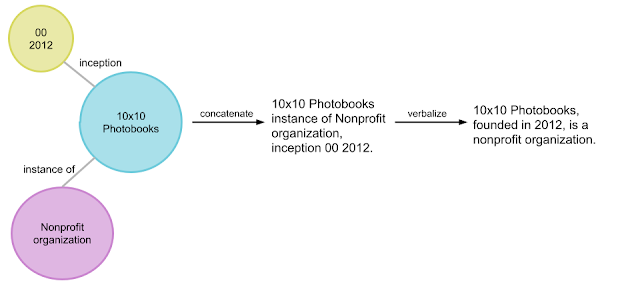
\includegraphics[width=0.5\linewidth,keepaspectratio]{llm47}
\end{center}	

{\tiny (Ref: KELM: Integrating Knowledge Graphs with Language Model Pre-training Corpora - Siamak Shakeri, Oshin Agarwal)}
\end{frame}




%%%%%%%%%%%%%%%%%%%%%%%%%%%%%%%%%%%%%%%%%%%%%%%%%%%%%%%%%%%%%%%%%%%%%%%%%%%%%%%%%%
\begin{frame}[fragile]\frametitle{}
\begin{center}
{\Large Leveraging LLM for Better KG}

\end{center}
\end{frame}

%%%%%%%%%%%%%%%%%%%%%%%%%%%%%%%%%%%%%%%%%%%%%%%%%%%%%%%%%%%%%%%%%%%%%%%%%%%%%%%%%%
%%%%%%%%%%%%%%%%%%%%%%%%%%%%%%%%%%%%%%%%%%%%%%%%%%%%%%%%%%%
\begin{frame}[fragile]\frametitle{How?}

\begin{itemize}
\item Organizations can take a systematic approach to generating a knowledge graph by first ingesting a standard ontology (like insurance risk) and using a large language model (LLM) like GPT-3 to create a script to generate and populate a graph database.cle.
\item The second step is to use an LLM as an intermediate layer to take natural language text inputs and create queries on the graph to return knowledge. 
\item The creation and search queries can be customized to the platform in which the graph is stored — such as Neo4j
\end{itemize}
\end{frame}

%%%%%%%%%%%%%%%%%%%%%%%%%%%%%%%%%%%%%%%%%%%%%%%%%%%%%%%%%%%
\begin{frame}[fragile]\frametitle{Steps}

\begin{center}
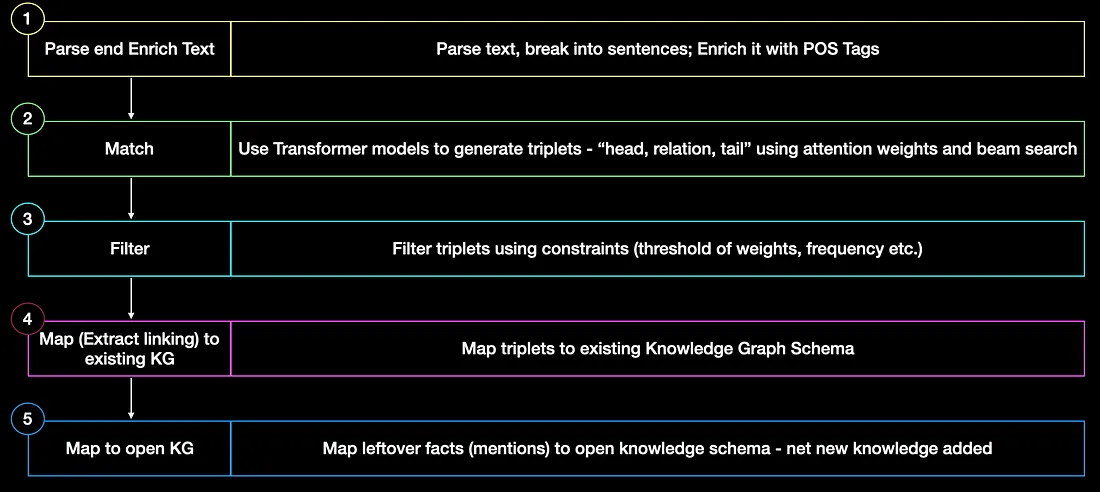
\includegraphics[width=0.5\linewidth,keepaspectratio]{llm52}
\end{center}	

{\tiny (Ref: Language Models are Open Knowledge Graphs .. but are hard to mine! - Nikhil Dharap)}
\end{frame}



%%%%%%%%%%%%%%%%%%%%%%%%%%%%%%%%%%%%%%%%%%%%%%%%%%%%%%%%%%%%%%%%%%%%%%%%%%%%%%%%%%
%%%%%%%%%%%%%%%%%%%%%%%%%%%%%%%%%%%%%%%%%%%%%%%%%%%%%%%%%%%
\begin{frame}[fragile]\frametitle{Steps}

\begin{itemize}
\item Studying the ontology and identifying entities and relations
\item Building a text prompt for LLM to generate schema and database for ontology
\item The text prompt should include a description of the ontology, the entities and relationships that were identified in step 1, and the desired schema and database structure. The description should be in natural language and should be easy for the LLM to understand. 
\item The text prompt should also include any constraints or requirements for the schema and database, such as data types, unique keys and foreign keys.
\item Once the text prompt is ready, it can be used as input to the LLM to generate the Cypher query for creating and populating the graph database.
\end{itemize}
\end{frame}



%%%%%%%%%%%%%%%%%%%%%%%%%%%%%%%%%%%%%%%%%%%%%%%%%%%%%%%%%%%
\begin{frame}[fragile]\frametitle{Work-flow}

\begin{center}
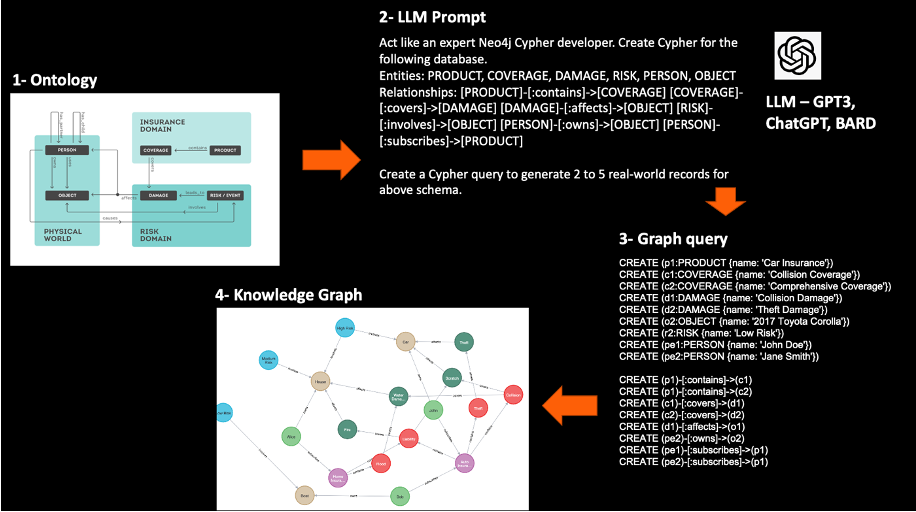
\includegraphics[width=\linewidth,keepaspectratio]{llm46}

{\tiny (Ref: How to use large language models and knowledge graphs to manage enterprise data - Dattaraj Rao, Persistent Systems)}
\end{center}
\end{frame}


%%%%%%%%%%%%%%%%%%%%%%%%%%%%%%%%%%%%%%%%%%%%%%%%%%%%%%%%%%%%%%%%%%%%%%%%%%%%%%%%%%
%%%%%%%%%%%%%%%%%%%%%%%%%%%%%%%%%%%%%%%%%%%%%%%%%%%%%%%%%%%
\begin{frame}[fragile]\frametitle{Pros and Cons}

\begin{itemize}
\item Standardization: By using a standard ontology, the organization can ensure that the data in the knowledge graph is consistent and standardized
\item Efficiency: Reduces the time and resources required to build the graph and ensures that the queries are syntactically and semantically correct.
\item Intuitive querying: Reduces the need for users to have a deep understanding of the graph structure and query language.
\item Productivity: Ability to update the knowledge graph as new data becomes available. The Cypher query can be modified to include new nodes and edges, and the updated query can be ingested into the graph database to add the new data. 
\end{itemize}
\end{frame}


%%%%%%%%%%%%%%%%%%%%%%%%%%%%%%%%%%%%%%%%%%%%%%%%%%%%%%%%%%%%%%%%%%%%%%%%%%%%%%%%%%
\begin{frame}[fragile]\frametitle{}
\begin{center}
{\Large Characteristics of KG + LLMs}

{\tiny (Ref: LinkedIn posts by Tony Seale)}
\end{center}
\end{frame}

%%%%%%%%%%%%%%%%%%%%%%%%%%%%%%%%%%%%%%%%%%%%%%%%%%%%%%%%%%%
\begin{frame}[fragile]\frametitle{Training data for GPT}

\begin{itemize}
\item Did you know that GPT is learning from web pages and that over 40\% of those web pages contain islands of JSON-LD?
\item You can reverse this relationship and use those islands to connect GPT's embeddings BACK to your own internal data!
\end{itemize}
	  
\end{frame}

%%%%%%%%%%%%%%%%%%%%%%%%%%%%%%%%%%%%%%%%%%%%%%%%%%%%%%%%%%%
\begin{frame}[fragile]\frametitle{Transformers as GNNs}

\begin{itemize}
\item Transformers analyse sentences by assigning importance to each word in relation to others, helping them predict or generate the next words in a sentence. 
\item This 'attention mechanism' evaluates pairwise interactions between all tokens in a sequence, and these interactions can be seen as edges in a complete graph. Thus, Transformers can be thought of as graph-based models where tokens represent nodes and attention weights represent edges.
\end{itemize}
	  
\end{frame}


%%%%%%%%%%%%%%%%%%%%%%%%%%%%%%%%%%%%%%%%%%%%%%%%%%%%%%%%%%%
\begin{frame}[fragile]\frametitle{Transparency and Explainability}

\begin{itemize}
\item  Language models, such as ChatGPT, can provide answers in a graph of interconnected nodes. 
\item By visualising these connections, we gain insights into their decision-making process, address biases, and ensure compliance with regulations.
\end{itemize}
	  
\end{frame}

%%%%%%%%%%%%%%%%%%%%%%%%%%%%%%%%%%%%%%%%%%%%%%%%%%%%%%%%%%%
\begin{frame}[fragile]\frametitle{Knowledge Management and Control}

\begin{itemize}
\item Connect the nodes generated by your language model to your organisation's Knowledge Graph. 
\item This integration grounds the model's output in established facts, enhancing accuracy while preventing the retrieval of outdated or incorrect information.
\end{itemize}
	  
\end{frame}

%%%%%%%%%%%%%%%%%%%%%%%%%%%%%%%%%%%%%%%%%%%%%%%%%%%%%%%%%%%
\begin{frame}[fragile]\frametitle{Alignment with Ontological Worldview}

\begin{itemize}
\item Leverage the concepts defined in your Knowledge Graph's ontology to constrain the language model. 
\item This alignment ensures that the model's output remains logically consistent with your organisation's world perspective.preventing the retrieval of outdated or incorrect information.
\end{itemize}
	  
\end{frame}

%%%%%%%%%%%%%%%%%%%%%%%%%%%%%%%%%%%%%%%%%%%%%%%%%%%%%%%%%%%
\begin{frame}[fragile]\frametitle{Alignment with Ontological Worldview}
\begin{itemize}
\item Leverage the concepts defined in your Knowledge Graph's ontology to constrain the language model. 
\item This alignment ensures that the model's output remains logically consistent with your organisation's world perspective.preventing the retrieval of outdated or incorrect information.
\end{itemize}
\end{frame}

%%%%%%%%%%%%%%%%%%%%%%%%%%%%%%%%%%%%%%%%%%%%%%%%%%%%%%%%%%%
\begin{frame}[fragile]\frametitle{Risk Assessment and Compliance}
\begin{itemize}
\item Knowledge graphs enable comprehensive risk assessment, empowering proactive identification of sensitive information, compliance risks, and ethical challenges. 
\item By leveraging this capability, you can mitigate potential issues before they escalate.
\end{itemize}
\end{frame}

%%%%%%%%%%%%%%%%%%%%%%%%%%%%%%%%%%%%%%%%%%%%%%%%%%%%%%%%%%%
\begin{frame}[fragile]\frametitle{Ethical and Fair AI}
\begin{itemize}
\item Knowledge graphs offer a rich and flexible platform to encode ethical guidelines and fairness constraints into an ontology that upholds your organisation's standards.
\item This ensures that the language model adheres to ethical principles and promotes fairness.
\end{itemize}
\end{frame}

%%%%%%%%%%%%%%%%%%%%%%%%%%%%%%%%%%%%%%%%%%%%%%%%%%%%%%%%%%%
\begin{frame}[fragile]\frametitle{Balancing Innovation and Risk Management in Today's Landscape.}
\begin{itemize}
\item In today's rapidly evolving landscape, organizations grapple with the challenge of balancing innovation and risk management. 
\item While language models like ChatGPT hold immense potential for boosting productivity and enhancing customer experiences, establishing robust governance frameworks is crucial to mitigate associated risks.
\end{itemize}
\end{frame}

%%%%%%%%%%%%%%%%%%%%%%%%%%%%%%%%%%%%%%%%%%%%%%%%%%%%%%%%%%%
\begin{frame}[fragile]\frametitle{Knowledge Graphs: A Safe Path Forward}
\begin{itemize}
\item Perhaps Knowledge graphs present a safe and effective approach for organisations looking to harness the power of language models.
\item By leveraging their capabilities, organisations can navigate the complex terrain of risk and governance while unlocking the benefits of AI-driven language models.
\end{itemize}
\end{frame}

%%%%%%%%%%%%%%%%%%%%%%%%%%%%%%%%%%%%%%%%%%%%%%%%%%%%%%%%%%%
\begin{frame}[fragile]\frametitle{Generalized or Specific}
\begin{itemize}
\item Large Language Models (LLMs) learn statistical approximations from text corpora, granting them generalisation, flexibility, and creativity. However, they also suffer from hallucinations, unreliability, and staleness.
\item On the other hand, databases offer accuracy, speed, and reliability but lack adaptability and intelligence.
\item Perhaps the key lies in bridging these two worlds, and that's where graphs come into play. By integrating LLMs with internal data through Knowledge Graphs, we can create a Working Memory Graph (WMG) that combines the strengths of both approaches in order to achieve a given task.
\item To build a WMG, the LLM processes a question and returns a graph of nodes using URLs as identifiers, these URLs link to ground truths stored in the organisation's Knowledge Graph. The WMG can also incorporate nodes representing conceptual understanding, establishing connections between the LLM's numerical vectors and the KG's ontological classes.
\end{itemize}
\end{frame}


%%%%%%%%%%%%%%%%%%%%%%%%%%%%%%%%%%%%%%%%%%%%%%%%%%%%%%%%%%%
\begin{frame}[fragile]\frametitle{KG + LLM @ Neo4j}
\begin{itemize}
\item https://github.com/neo4j/NaLLM
\item To explore, develop, and showcase practical uses of these LLMs in conjunction with Neo4jdata science algorithms, as this strategy could yield substantial breakthroughs for their businesses.
\item Expect to enhance the accuracy, transparency, and predictability of the model output and open up new use-cases both for using LLMs as well as databases.
\item Real-world use-cases:

	\begin{itemize}
	\item Natural Language Interface to a Knowledge Graph, allowing you to “talk to your database” ie generate database queries based on the user question and the inferred schema of the database.
	\item Creating a Knowledge Graph from Unstructured Data, LLMs can decipher entities, discern relationships, and eliminate redundancies by recognizing duplicates.
	\end{itemize}

\end{itemize}
\end{frame}


%%%%%%%%%%%%%%%%%%%%%%%%%%%%%%%%%%%%%%%%%%%%%%%%%%%%%%%%%%%%%%%%%%%%%%%%%%%%%%%%%%
\begin{frame}[fragile]\frametitle{}
\begin{center}
{\Large Conclusions}

\end{center}
\end{frame}

%%%%%%%%%%%%%%%%%%%%%%%%%%%%%%%%%%%%%%%%%%%%%%%%%%%%%%%%%%%%%%%%%%%%%%%%%%%%%%%%%%
%%%%%%%%%%%%%%%%%%%%%%%%%%%%%%%%%%%%%%%%%%%%%%%%%%%%%%%%%%%
\begin{frame}[fragile]\frametitle{Benefits of Combining Knowledge Graphs and LLMs}

\begin{itemize}
\item Centralized source of accurate knowledge
\item Structured knowledge fusion of information in different formats
\item Increased informative value of collected data
\item Gives LLMs a human reference frame of the real-world
\end{itemize}

\end{frame}


%%%%%%%%%%%%%%%%%%%%%%%%%%%%%%%%%%%%%%%%%%%%%%%%%%%%%%%%%%%
\begin{frame}[fragile]\frametitle{Conclusions}
\begin{itemize}
\item Incorporating graph-based Knowledge Graphs as support mechanisms for LLMs like ChatGPT can overcome their limitations in the enterprise context. 
\item By leveraging Knowledge Graphs, organizations can improve AI accuracy and relevance, leading to better data comprehension, refined compliance procedures, and accelerated research and development. 
\item Chief Information Officers should explore the potential of applying LLMs to internal data stores and constructing knowledge graphs through graph data science algorithms, as this strategy could yield substantial breakthroughs for their businesses.
\end{itemize}
\end{frame}


%%%%%%%%%%%%%%%%%%%%%%%%%%%%%%%%%%%%%%%%%%%%%%%%%%%%%%%%%%%
\begin{frame}[fragile]\frametitle{References}
\begin{itemize}
\item Knowledge Graphs \& LLMs: Fine-Tuning Vs. Retrieval-Augmented Generation - Tomaz Bratanic
\item Building knowledge graphs from unstructured data with OpenAI by Priyanka Shah
\item LLM’s Closing the KG Gap - Dean Allemang
\item The Future of Knowledge Graphs in a World of Large Language Models - Denny Vrandecic
\item Generating Company Recommendations using Large Language Models and Knowledge Graphs by Mike Tung
\item Large Language Model = Knowledge Graph Store? Yes, by Fine-Tuning LLM With KG - Peter Lawrence
\item Knowledge Graphs + Large Language Models = The ability for users to ask their own questions? - Peter Lawrence
\item Automatic Knowledge Graphs: The Impossible Grail - Patrick Meyer
\item Project NaLLM - https://github.com/neo4j/NaLLM
\item KELM: Integrating Knowledge Graphs with Language Model Pre-training Corpora 
\item How to use large language models and knowledge graphs to manage enterprise data 
\item Enhancing Large Language Models with Graph-based Knowledge Graphs: Overcoming Limitations and Unlocking Enterprise Potential - Nicholas Moss
\end{itemize}
\end{frame}
